\section{The Domino compiler}
\label{s:compiler}

The \pktlanguage compiler translates \pktlanguage programs to \absmachine
targets. The compiler provides an {\em all-or-nothing model}: if compilation
succeeds, the program will run at line rate on the target with packet
transaction semantics. Otherwise, if the program cannot run at line rate, it
will not compile. This all-or-nothing model trades off diminished
programmability for guaranteed line-rate performance, in contrast to software
routers that provide greater flexibility, but lower and unpredictable run-time
performance~\cite{dobrescu2012}.

The \pktlanguage compiler has three passes (Figure~\ref{fig:passes}), which we
illustrate using the flowlet switching example.  \textit{Preprocessing}
(\S\ref{ss:preprocessing}) simplifies packet transactions into a simpler
three-address code form~\cite{tac}.
\textit{Pipelining} (\S\ref{ss:pipelining}) transforms preprocessed code into
code for a \textit{Pipelined Virtual Router Machine (PVSM)}, an intermediate
representation that models a router pipeline with no computational or resource
limits. \textit{Code generation} (\S\ref{ss:code_gen}) transforms this
intermediate representation into configuration for a \absmachine machine, given
the machine's computational and resource limits (\S\ref{s:atomConstraints}),
and rejects the program if it can not run at line rate.  The \pktlanguage
compiler uses many existing compilation techniques, but adapts
them in important ways for line-rate routers (\S\ref{ss:related_compiler}).

\begin{figure}[!t]
  \centering
  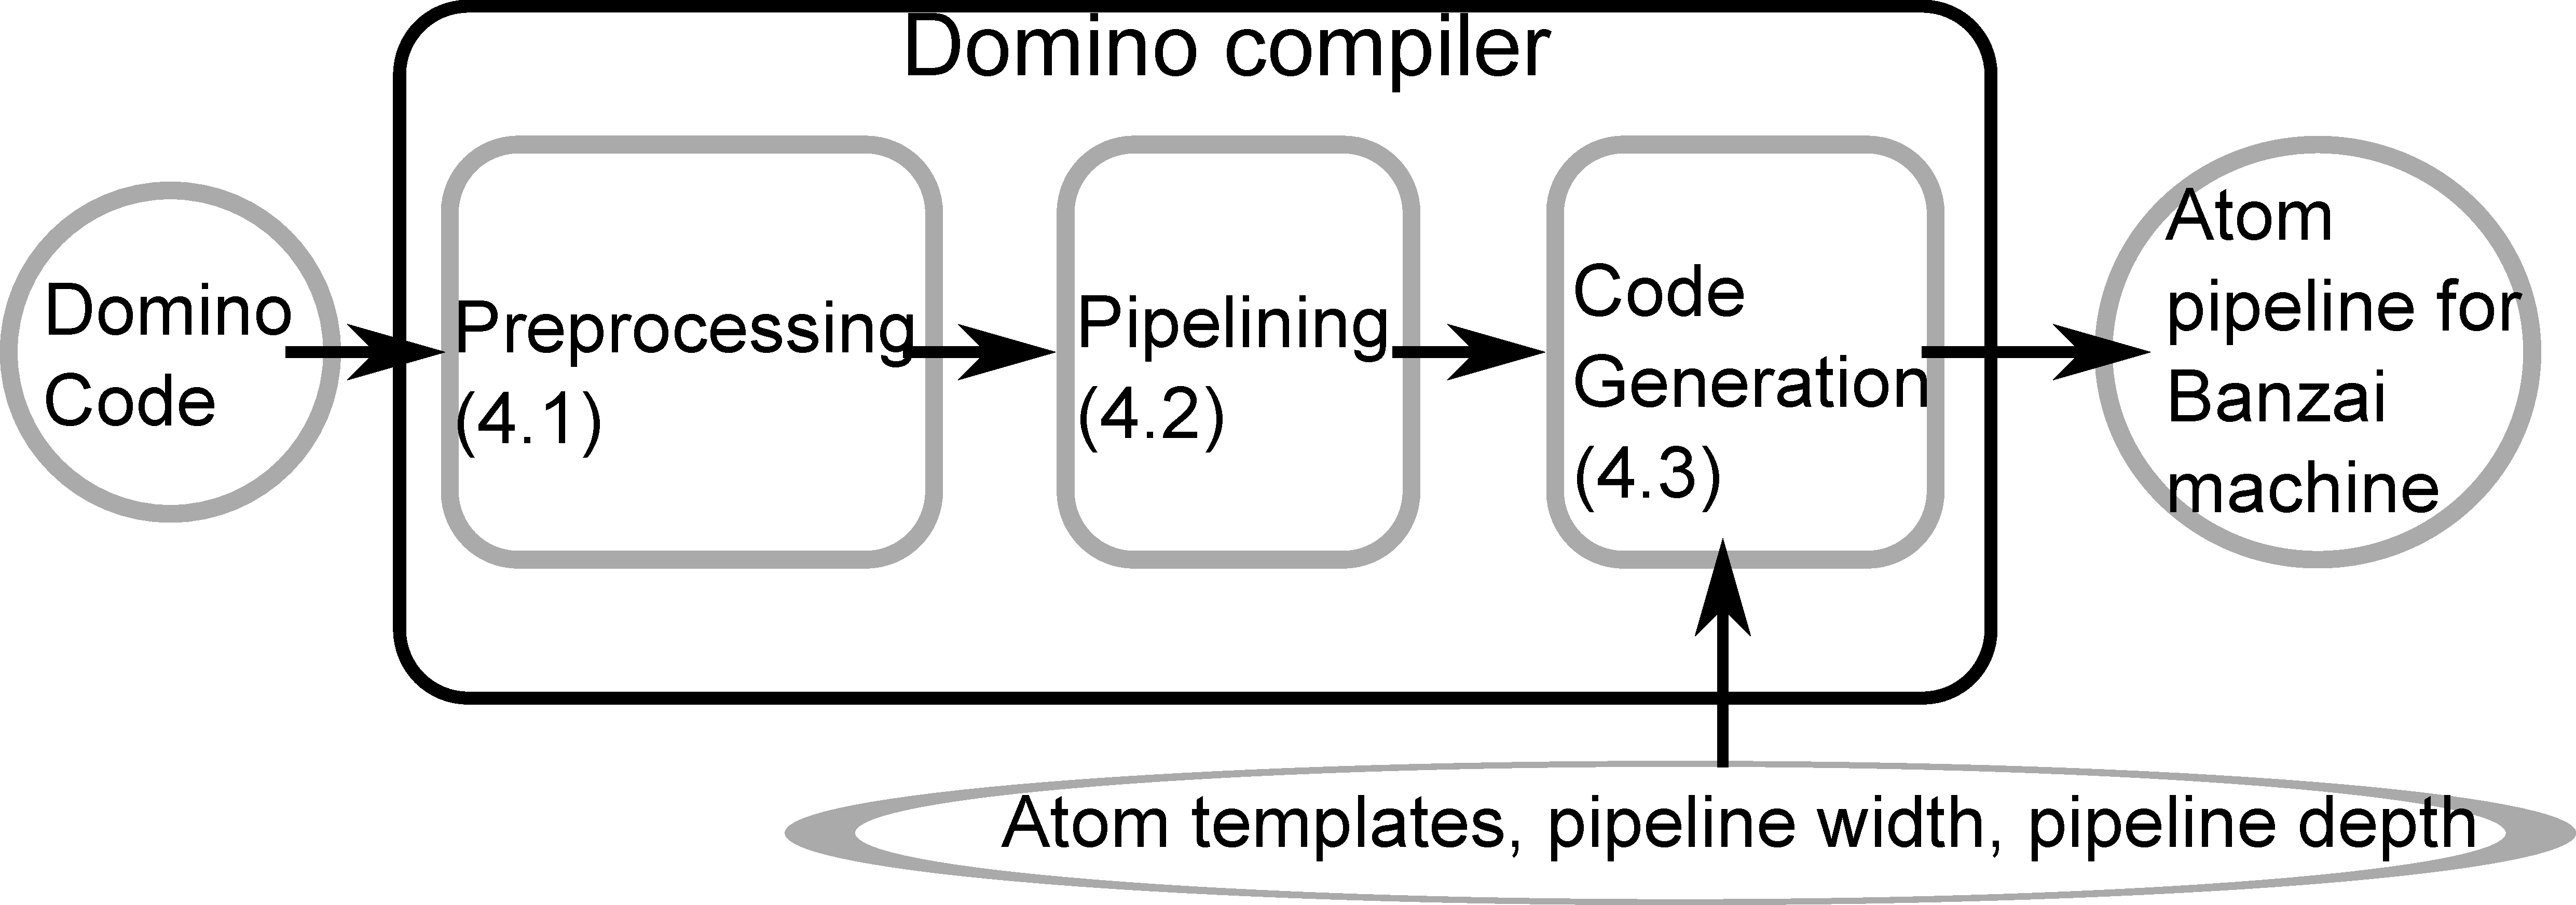
\includegraphics[width=0.75\columnwidth]{domino_compiler.pdf}
  \caption{Passes in the \pktlanguage compiler}
  \label{fig:passes}
\end{figure}

\subsection{Preprocessing}
\label{ss:preprocessing}

\medskip
\noindent
\textbf{Branch removal.} A packet transaction's body can contain (potentially
nested) branches (e.g., Lines~\ref{line:ifStart} to \ref{line:ifEnd} in
Figure~\ref{fig:flowlet_code}).  Branches alter control flow and complicate
dependency analysis, i.e.,  whether a statement should precede another.  We
transform branches into conditional assignments, starting from the innermost
\texttt{if} and proceeding outwards (Figure~\ref{fig:if_convert}).  This turns
the transaction body into straight-line code with no branches, which simplifies
dependency analysis during pipelining (\S\ref{ss:pipelining}).

\medskip
\noindent
\textbf{Rewriting state variable operations.} We now identify state variables
in a packet transaction, e.g., \texttt{last\_time} and \texttt{saved\_hop} in
Figure~\ref{fig:flowlet_code}.  For each state variable, we create a
\textit{read flank} to read the variable into a temporary packet field.
For an array, we also move the index expression into the read flank using the
fact that only one array index is accessed per packet (\S\ref{ss:constraints}).
Within the packet transaction, we replace the state variable with the temporary
packet field, and create a \textit{write flank} to write this temporary packet
field back to the state variable~(Figure~\ref{fig:stateful_flanks}). After
this, the only operations on state variables are reads and writes; all
arithmetic happens on packet fields. Restricting stateful operations simplifies
handling of state during pipelining (\S\ref{ss:pipelining}).

\medskip
\noindent
\textbf{Converting to static single-assignment form.} We next convert the code
to static single-assignment form (SSA)~\cite{ssa}, where every packet field is
assigned exactly once. We do this by replacing every assignment to a packet
field with a new packet field and propagating this until the next assignment to
the same field~(Figure~\ref{fig:ssa}) .  Because fields are assigned once, SSA
removes Write-After-Read and Write-After-Write dependencies.  Only
Read-After-Write dependencies remain during pipelining (\S\ref{ss:pipelining}).

\medskip
\noindent
\textbf{Flattening to three-address code.} Three-address code is a
representation where all instructions are either reads/writes into state
variables or operations on packet fields of the form \texttt{pkt.f1 = pkt.f2 op
pkt.f3}, where \texttt{op} can be an arithmetic, logical, relational, or
conditional \footnote{Conditional operations alone have four arguments.}
operator.  We also allow either one of {\tt pkt.f2} or {\tt pkt.f3} to be an
intrinsic function call.  To convert to three-address code, we flatten
expressions that are not in three-address code using
temporary packet fields, e.g., {\tt pkt.tmp2} in Figure~\ref{fig:three_address}.

Flattening to three-address code breaks down
statements in the packet transaction into a much simpler form that is closer
to the atoms available in the \absmachine machine. For instance, there are no
nested expressions. The simpler form of three-address code statements
makes it easier to map them one-to-one to atoms during code generation (\S\ref{ss:code_gen}).
%\ac{I don't think it's any easier conceptually 
%since we are using sketch to find the mapping. But it might be easier to write 
%the mapping sketch code.}
% I agree. That's what I meant here. E.g., the stateless codelets correspond directly to the instructions available.
% Otherwise, we might have to break up codelets into multiple atoms and worry about how to do that.

% Anirudh->Alvin: Can you check the above paragraph?

\subsection{Pipelining}
\label{ss:pipelining}
At this point, the preprocessed code is still one sequential code block.
Pipelining turns this sequential code block into a pipeline of
\textit{codelets}, where each codelet is a sequential block of three-address
code statements. This codelet pipeline corresponds to an intermediate
representation we call the \textit{Pipelined Virtual Router Machine (PVSM)}.
PVSM has no computational or resource limits, analogous to intermediate
representations for CPUs~\cite{llvm} that have infinite virtual
registers. Later, during code generation, we map these codelets to atoms
available in a \absmachine machine while respecting its constraints.

\new{
We create PVSM's codelet pipeline using the steps below.
\begin{CompactEnumerate}
  \item Create a graph with one node for each statement in the preprocessed code.
  \item Now, add {\em stateful dependencies} by adding a pair of edges between
    the read and write flanks of the same state variable, e.g., in
    Figure~\ref{fig:partitioning_before}, the node pair {\tt pkt.last\_time =
    last\_time[pkt.id]} and {\tt last\_time[pkt.id] = pkt.arrival}. Because of
    preprocessing, all stateful operations are paired up as read and write flanks.
    Hence, there is no risk of a ``stranded'' stateful operation.
  \item Now, add {\em stateless dependencies} by adding an edge from any node
    that writes a packet variable to any node that reads the same packet variable,
    e.g., from {\tt pkt.tmp = pkt.arrival - pkt.last\_time} to {\tt pkt.tmp2 =
    pkt.tmp > THRESH} in Figure~\ref{fig:partitioning_before}. We only check read-after-write dependencies because
    write-after-read and write-after-write dependencies don't exist after SSA, and
    we eliminate control dependencies~\cite{ssa} through branch removal.
  \item Generate strongly connected components (SCCs) of this dependency graph
    and condense them into a directed acyclic graph (DAG). This captures the notion that all
    operations on a state variable must be confined to one codelet/atom because
    state cannot be shared between atoms. Figure~\ref{fig:partitioning_after}
    shows the DAG produced by condensing Figure~\ref{fig:partitioning_before}.
  \item Schedule the resulting DAG by creating a new pipeline stage when one
    node depends on another. This results in the codelet pipeline
    shown in Figure~\ref{fig:flowlet_pipeline}.\footnote{We refer to this both
    as a codelet and an atom pipeline because codelets map one-to-one atoms
  (\S\ref{ss:code_gen}).}
% Ditching ref to crit. path scheduling.
\end{CompactEnumerate}
}
%\footnote{An instruction A is control
%    dependent on a preceding instruction B if the outcome of B determines
%    whether A should be executed or not.}
%The codelet pipeline implements the packet transaction on a router pipeline
%with no computational or resource constraints. We handle these next.

\begin{figure*}[!t]
  \hspace{-0.4in}
  \begin{minipage}{0.55\textwidth}
  \begin{small}
  \begin{lstlisting}[style=customcscriptsize, numbers=none, frame=none]
  if (@\textcolor{blue}{pkt.arrival - last\_time[pkt.id] > THRESH}@) {
    saved_hop[pkt.id] = pkt.new_hop;
  }
  \end{lstlisting}
  \end{small}
  \end{minipage}
%  
  \hspace{-0.3in}
  $\Longrightarrow$ 
  \hspace{-0.3in}
%  
  \begin{minipage}{0.6\textwidth}
  \begin{small}
  \begin{lstlisting}[style=customcscriptsize, numbers=none, frame=none]
  @\textcolor{blue}{pkt.tmp = pkt.arrival - last\_time[pkt.id]  > THRESH}@;
  saved_hop[pkt.id] = @\textcolor{blue}{pkt.tmp}@  @\textcolor{magenta}{// Rewritten}@
                      ? pkt.new_hop
                      : saved_hop[pkt.id];
  \end{lstlisting}
  \end{small}
  \end{minipage}
%\vspace{-.2in}
\caption{Branch removal}
\label{fig:if_convert}
\end{figure*}

\begin{figure*}[!t]
  \begin{minipage}{0.43\textwidth}
  \begin{small}
  \begin{lstlisting}[style=customcscriptsize, numbers=none, frame=none]
pkt.id = hash2(pkt.sport,
               pkt.dport)
         % NUM_FLOWLETS;
...
@\textcolor{blue}{last\_time[pkt.id] = pkt.arrival;}@
...
  \end{lstlisting}
  \end{small}
  \end{minipage}
%  
  \hspace{-0.5in}
  $\Longrightarrow$ 
  \hspace{-0.2in}
%  
  \begin{minipage}{0.61\textwidth}
  \begin{small}
  \begin{lstlisting}[style=customcscriptsize, numbers=none, frame=none]
pkt.id = hash2(pkt.sport,           @\textcolor{magenta}{// Read flank}@
               pkt.dport)
         % NUM_FLOWLETS;
pkt.last_time = last_time[pkt.id];  @\textcolor{magenta}{// Read flank}@
...
@\textcolor{blue}{pkt.last\_time = pkt.arrival;}@       @\textcolor{magenta}{// Rewritten}@
...
last_time[pkt.id] = pkt.last_time;  @\textcolor{magenta}{// Write flank}
  \end{lstlisting}
  \end{small}
  \end{minipage}
  \caption{Rewriting state variable operations}
\label{fig:stateful_flanks}
\end{figure*}

\begin{figure*}[!t]
  \begin{minipage}{\textwidth}
  \begin{minipage}{0.4\textwidth}
  \begin{small}
  \begin{lstlisting}[style=customcscriptsize, numbers=none, frame=none]
@\textcolor{blue}{pkt.id}@ = hash2(pkt.sport,
              pkt.dport)
              % NUM_FLOWLETS;
@\textcolor{blue}{pkt.last\_time}@ = last_time[@\textcolor{blue}{pkt.id}@];
...
@\textcolor{blue}{pkt.last\_time}@ = pkt.arrival;
last_time[@\textcolor{blue}{pkt.id}@] = @\textcolor{blue}{pkt.last\_time}@;
  \end{lstlisting}
  \end{small}
  \end{minipage}
 % 
  %\hspace{-0.1in}
  $\Longrightarrow$
  \hspace{-0.2in}
%
  \begin{minipage}{0.6\textwidth}
  \begin{small}
  \begin{lstlisting}[style=customcscriptsize, numbers=none, frame=none]
@\textcolor{blue}{pkt.id0}@ = hash2(pkt.sport,            @\textcolor{magenta}{// Rewritten}@ @\label{line:assign}@
               pkt.dport)
               % NUM_FLOWLETS;  
@\textcolor{blue}{pkt.last\_time0}@ = last_time[@\textcolor{blue}{pkt.id0}@];  @\textcolor{magenta}{// Rewritten}@
...
@\textcolor{blue}{pkt.last\_time1}@ = pkt.arrival;         @\textcolor{magenta}{// Rewritten}@
last_time[@\textcolor{blue}{pkt.id0}@] = @\textcolor{blue}{pkt.last\_time1}@;  @\textcolor{magenta}{// Rewritten}@
  \end{lstlisting}
  \end{small}
  \end{minipage}
  \caption[title]{Converting to static single-assignment form}
  \label{fig:ssa}
\end{minipage}
\end{figure*}


\begin{figure*}[!t]
\begin{minipage}{\textwidth}
\begin{lstlisting}[style=customc]
pkt.id            = hash2(pkt.sport, pkt.dport) % NUM_FLOWLETS; @\label{line:id}@
pkt.saved_hop     = saved_hop[pkt.id]; @\label{line:stateRead}@
pkt.last_time     = last_time[pkt.id];
pkt.new_hop       = hash3(pkt.sport, pkt.dport, pkt.arrival) % NUM_HOPS; @\label{line:newhop}@
pkt.tmp           = pkt.arrival - pkt.last_time;
pkt.tmp2          = pkt.tmp > THRESH;
pkt.next_hop      = pkt.tmp2 ? pkt.new_hop : pkt.saved_hop;
saved_hop[pkt.id] = pkt.tmp2 ? pkt.new_hop : pkt.saved_hop; @\label{line:stateWrite}@
last_time[pkt.id] = pkt.arrival;
\end{lstlisting}
\caption[title2]{Flowlet switching in three-address
code. Lines~\ref{line:id} and \ref{line:newhop} are flipped relative
to Figure~\ref{fig:flowlet_code} because {\tt pkt.id} is an array index expression and is
moved into the read flank.}
\label{fig:three_address}
\end{minipage}
\vspace{-0.3cm}
\end{figure*}

%TODO: This figure is OK, but it could be improved.
\begin{figure*}[!t]
\begin{subfigure}{0.5\columnwidth}
  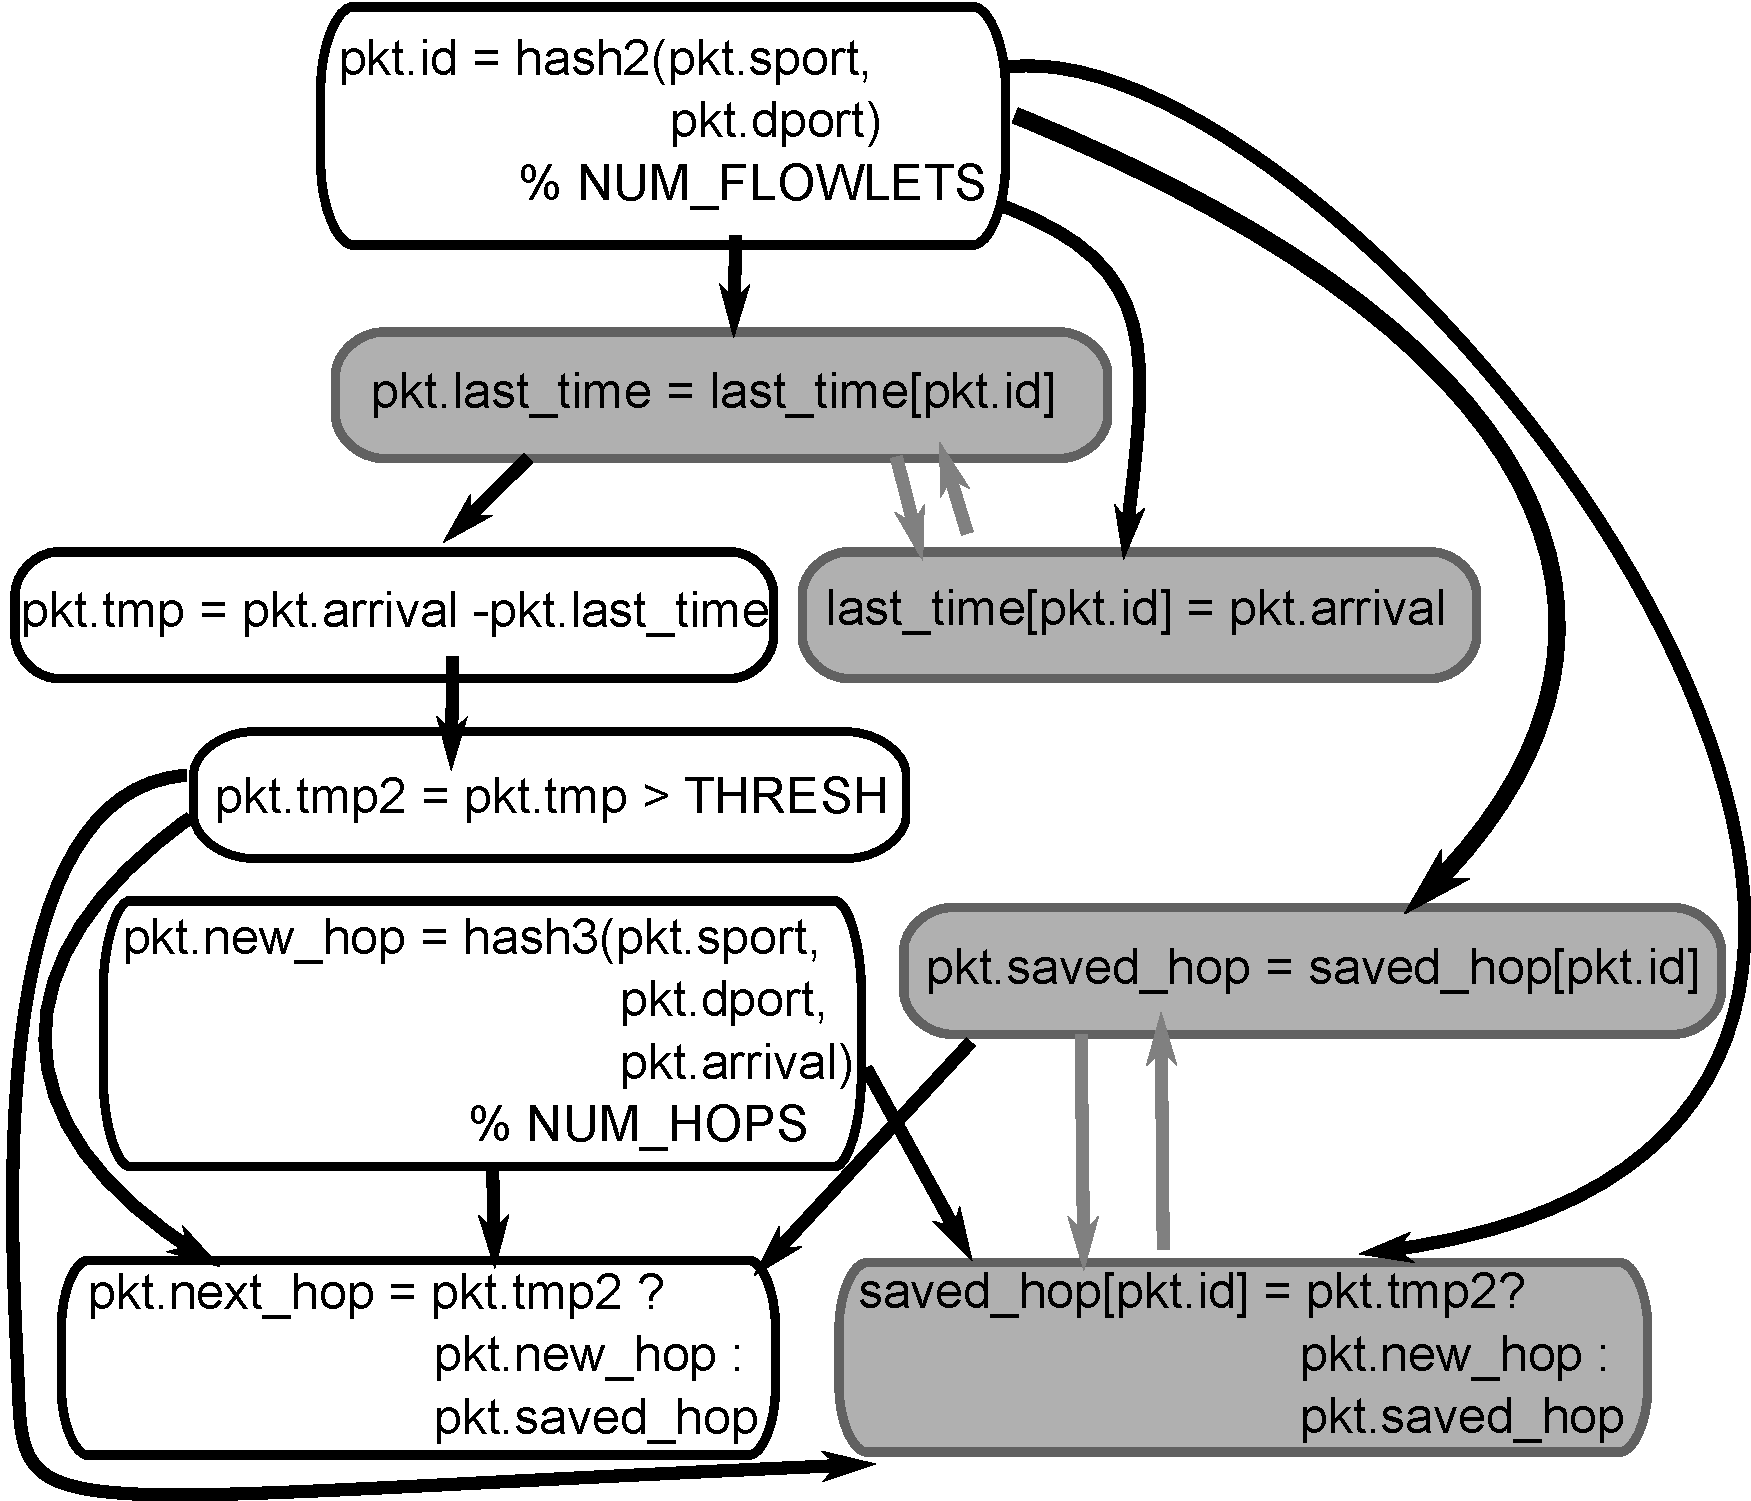
\includegraphics[width=0.98\columnwidth]{domino_deps.pdf}
  \caption{Stateless dependencies in black, stateful in gray.}
  \label{fig:partitioning_before}
\end{subfigure}
\textbf{$\Longrightarrow$ }
\begin{subfigure}{0.5\columnwidth}
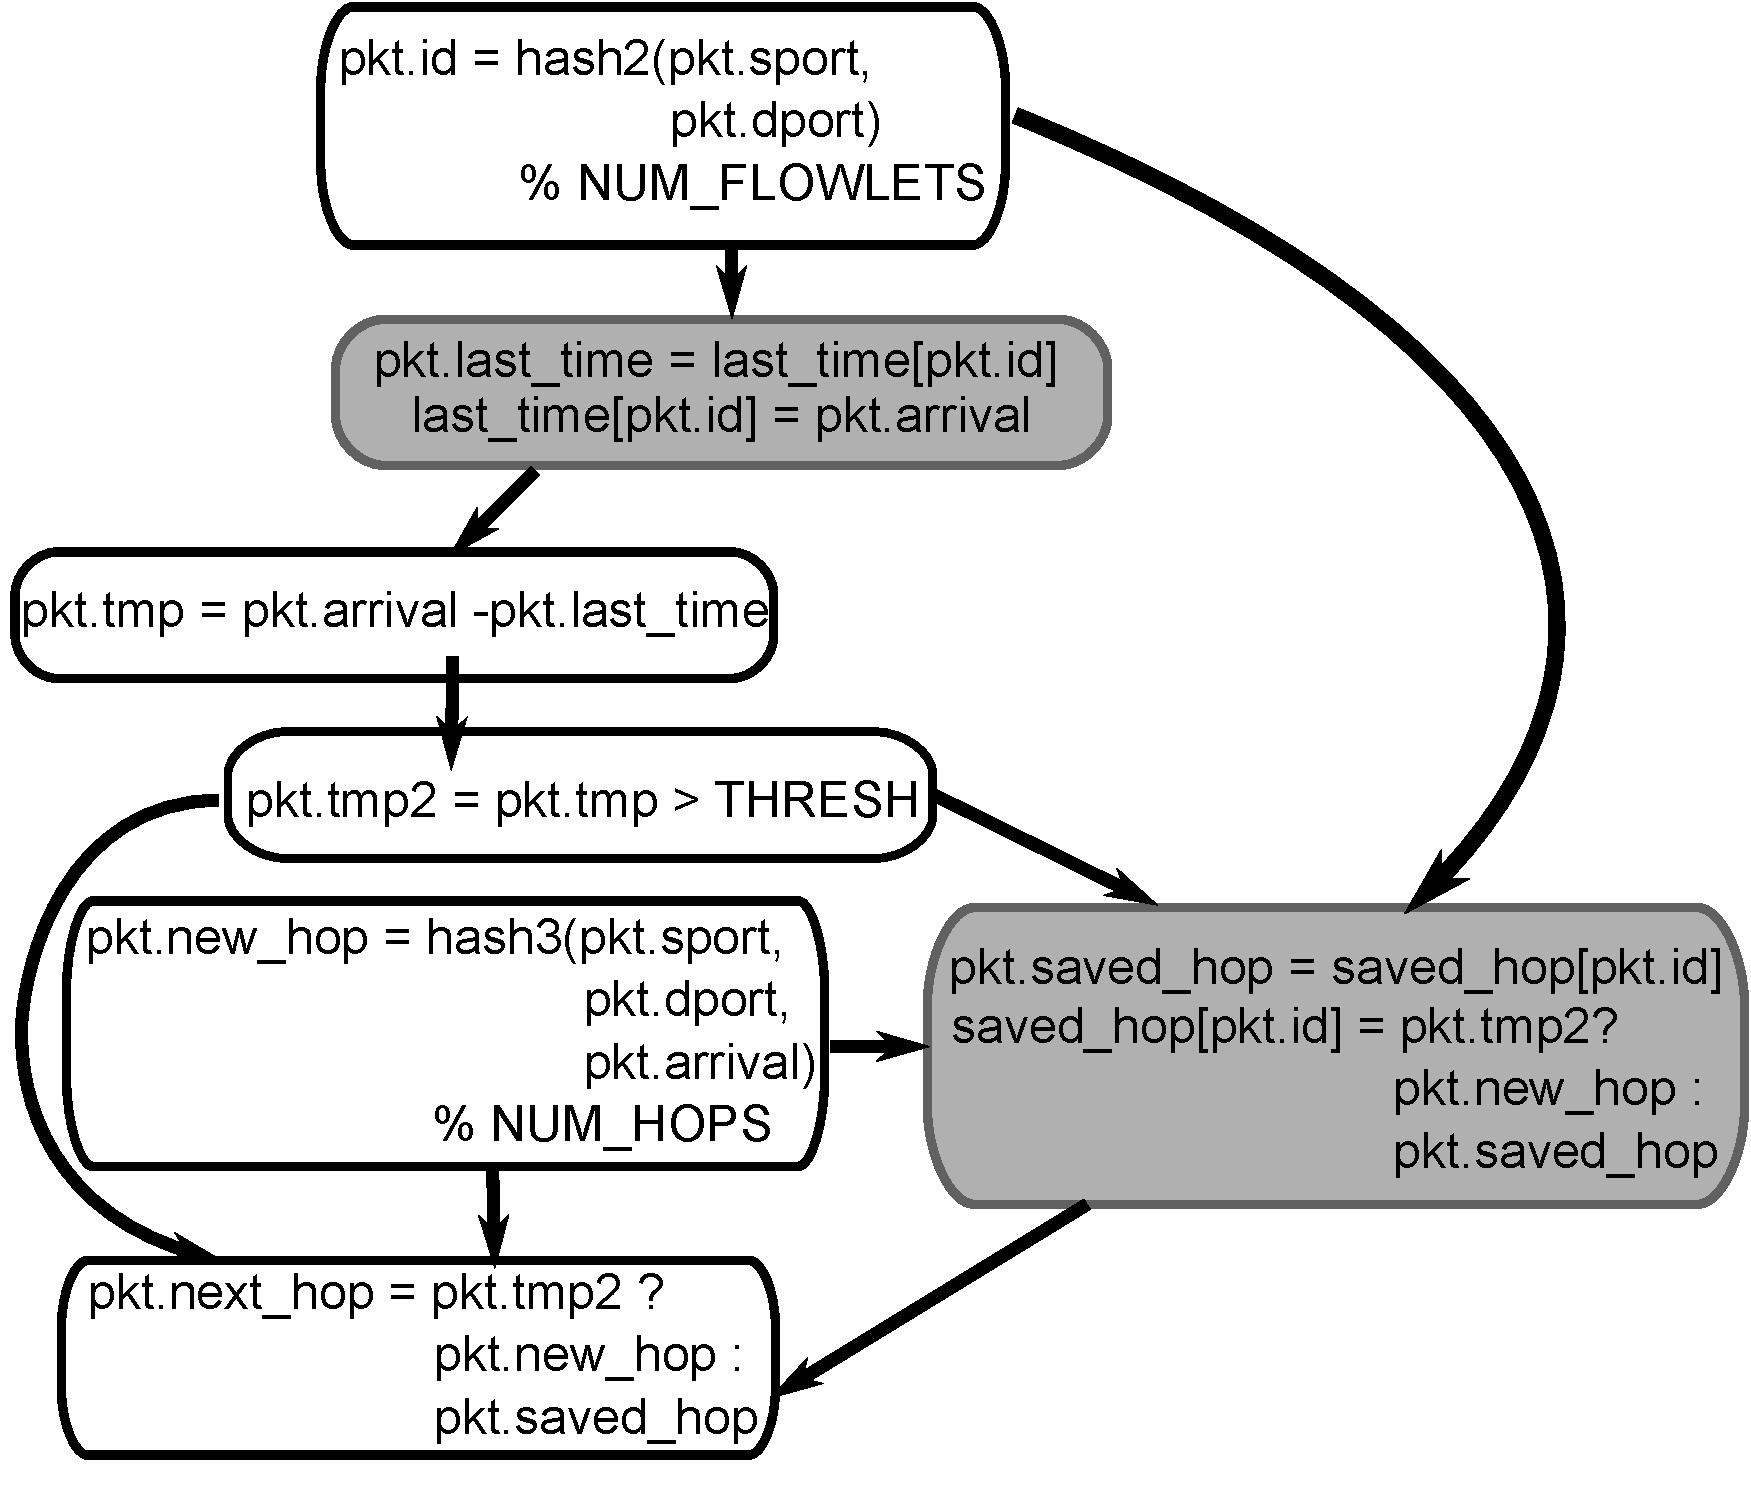
\includegraphics[width=0.98\columnwidth]{domino_scc.pdf}
\caption{DAG after condensing SCCs.}
\label{fig:partitioning_after}
\end{subfigure}
\caption{Dependency graphs before and after condensing strongly connected components}
\label{fig:pipelining}
\end{figure*}




\subsection{Code generation}
\label{ss:code_gen}

To determine if a codelet pipeline can be compiled to a \absmachine machine, we
consider two constraints specified by any \absmachine machine
(\S\ref{s:atomConstraints}).  Resource limits specify the number of atoms in a
stage (pipeline width) and number of stages (pipeline depth), while
computational limits specify the atom templates provided by a \absmachine
machine.

\medskip
\noindent
\textbf{Resource limits.} To handle resource limits, we scan each pipeline
stage in the codelet pipeline starting from the first to check for pipeline
width violations. If we violate the pipeline width, we insert as many new
stages as required and spread codelets evenly across these stages.  We continue
until the number of codelets in all stages is under the pipeline width,
rejecting the program if we exceed the pipeline depth.

\medskip
\noindent
\textbf{Computational limits.} Next, we determine if each codelet in the pipeline
can be mapped to atoms provided by the \absmachine machine. In general,
codelets have multiple three-address code statements that need to execute
atomically. For instance, updating the state variable \texttt{saved\_hop} in
Figure~\ref{fig:flowlet_pipeline} requires a read followed by a conditional
write.  It is not apparent whether such codelets can be mapped to an available
atom. We develop a new technique to determine the implementability of a codelet,
given an atom template.

Each atom template has a set of configuration parameters, where the parameters
determine the atom's behavior.  For instance, Figure~\ref{fig:alu_diag} shows
an atom that can perform stateful addition or subtraction, depending on the
configuration parameters {\tt choice} and {\tt constant}.  Each codelet can be
viewed as a functional specification of the atom.  With that in mind, the
mapping problem is equivalent to searching for values of the atom's configuration
parameters that result in the atom implementing the codelet.

We use the SKETCH program synthesizer~\cite{sketch_asplos} for this purpose, as
the atom templates can be easily expressed using SKETCH. SKETCH also
provides efficient search algorithms and has been used for similar purposes in
other domains~\cite{lifejoin, qbs}. As an
illustration, assume we want to map the codelet {\tt x=x+1} to the atom
template shown in Figure~\ref{fig:alu_in_sketch}. SKETCH will search for
possible parameter values so that the resulting atom is functionally identical
to the codelet, for all possible input values of {\tt x} up to a certain bound. 
In this case, SKETCH
finds the solution with {\tt choice=0} and {\tt constant=1}.  In contrast, if
the specification is the codelet {\tt x=x*x}, SKETCH will return
an error as no parameters exist.

Using program synthesis for code generation frees the compiler developer from implementing
custom code generators for different \absmachine machines.
Instead, the
compiler developer only has to express the \absmachine machine's
atom templates using SKETCH, and the SKETCH synthesizer automatically maps
codelets to atoms.

%%To minimize search time, the range
%%of possible inputs and parameter values need to be specified in the template
%%(e.g., all 8 bit integers), and our experiments show that the search finishes
%%quickly, taking 10 secs at most.

\subsection{Related compiler techniques}
\label{ss:related_compiler}
Table~\ref{tab:prior_compiler} shows the relationship between \pktlanguage's
compilation techniques and prior work. The use of Strongly Connected Components
(SCCs) is inspired by software pipelining for VLIW
architectures~\cite{software_pipelining}. The size of the largest SCC affects
the {\em maximum throughput} of the pipelined loop in software pipelining. For
\pktlanguage, it affects the {\em circuit area} of the atom required to run a
program at line rate. \pktlanguage trades off an increase in space for
line-rate performance.

Program synthesis was used for code generation in
Chlorophyll~\cite{chlorophyll}.  Code generation for \pktlanguage also shares
similar goals to technology mapping~\cite{micheli} and
instruction selection~\cite{dragonbook}.  However, prior work maps a code sequence
to \textit{multiple} instructions/tiles, using heuristics to minimize
instruction count. Domino's problem is simpler: we map each codelet to a single
atom using SKETCH.  The simpler problem allows a non-heuristic solution: if
there is any way to map the codelet to an atom, SKETCH will find it.

Branch removal resembles If-Conversion~\cite{if_conversion}, a
technique used in vectorizing compilers. This procedure is easier in Domino
because there is no backward control transfer ({\tt goto}, {\tt break},
{\tt continue}).

\begin{table}[!t]
  \centering
  \begin{small}
    \begin{tabular}{|p{0.2\textwidth}|p{0.2\textwidth}|p{0.4\textwidth}|}
  \hline
  Technique & Prior Work & Differences \\
  \hline
  Conversion to straight-line code & If-Conversion~\cite{if_conversion} & No backward control flow (gotos, break, continue) \\
  \hline
  SSA & Cytron et al.~\cite{ssa} & SSA runs on straight-line code with no branches \\
  \hline
  Strongly Connected Components & Lam~\cite{software_pipelining} & Scheduling in space vs. time \\
  \hline
  Code generation using program synthesis & Chlorophyll~\cite{chlorophyll}, technology mapping~\cite{micheli}, instruction selection~\cite{dragonbook} & Optimal vs. best-effort mapping, One-to-one mapping vs. one-to-many mapping \\
  \hline
  \end{tabular}
  \end{small}
  \caption{Domino's compiler in relation to prior work}
  \label{tab:prior_compiler}
\end{table}
